% 第 16 题直三棱柱图：按固定源 PDF 矢量路径换算（1 pt → 0.03515 cm）。
% 原点取 A 点（源页 (666.91, 770.95) pt），y 向上。
% 上底面 A₁B₁C₁（C₁ 在后）、下底面 ABC（C 在后）；D 为 AB 中点、E 为 BC 中点、F 在棱 B₁B 上。
% 实线 8 段：下底 AB、侧棱 AA₁/BB₁、上底 B₁A₁ 与 A₁C₁/C₁B₁、辅助线 DB₁ 与 AF；
% 虚线 5 段：被遮挡的 CA/CB/CC₁、C₁F、折线 D–E–B₁（V 形，两段均取虚线）。
% 注：源内 F 实测位于自 B₁ 起约 0.446 倍棱长处（非中点；题面仅要求「在 B₁B 上」，照源复刻）。
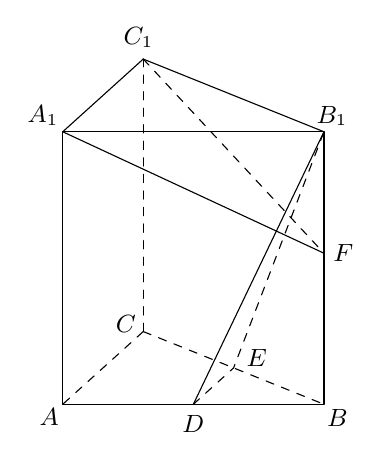
\begin{tikzpicture}[line cap=round,line join=round,font=\small,x=0.03515cm,y=0.03515cm]
% ===== 实线（8 段）=====
\draw (0,0)--(94.36,0);            % A–B
\draw (0,98.44)--(29.08,124.71);   % A₁–C₁
\draw (29.08,124.71)--(94.36,98.44); % C₁–B₁
\draw (94.36,0)--(94.36,98.44);    % B–B₁（过 F）
\draw (94.36,98.44)--(0,98.44);    % B₁–A₁
\draw (0,98.44)--(0,0);            % A₁–A
\draw (47.18,0)--(94.36,98.44);    % D–B₁
\draw (0,98.44)--(94.36,54.57);    % A–F
% ===== 虚线（5 段）=====
\draw[dash pattern=on 2.99pt off 2.99pt] (29.08,26.27)--(94.36,0);    % C–B
\draw[dash pattern=on 2.99pt off 2.99pt] (29.08,26.27)--(0,0);        % C–A
\draw[dash pattern=on 2.99pt off 2.99pt] (29.08,26.27)--(29.08,124.71); % C–C₁
\draw[dash pattern=on 2.99pt off 2.99pt] (29.08,124.71)--(94.36,54.57); % C₁–F
\draw[dash pattern=on 2.99pt off 2.99pt] (47.18,0)--(61.72,13.13)--(94.36,98.44); % D–E–B₁
% ===== 标注（照源字框中心，显式坐标）=====
\node[anchor=center,inner sep=0] at (-7.12,104.33) {\(A_{1}\)};
\node[anchor=center,inner sep=0] at (97.26,104.15) {\(B_{1}\)};
\node[anchor=center,inner sep=0] at (27.35,132.47) {\(C_{1}\)};
\node[anchor=center,inner sep=0] at (-4.88,-4.76) {\(A\)};
\node[anchor=center,inner sep=0] at (99.23,-4.93) {\(B\)};
\node[anchor=center,inner sep=0] at (22.77,28.94) {\(C\)};
\node[anchor=center,inner sep=0] at (47.12,-6.97) {\(D\)};
\node[anchor=center,inner sep=0] at (70.05,16.55) {\(E\)};
\node[anchor=center,inner sep=0] at (101.38,54.56) {\(F\)};
\end{tikzpicture}
